% ============================================================
% ACM40960 Poster -- Explainable ML for Irish Residential
% Energy Retrofit Prioritisation Using BER Data
%
% Compile on Overleaf (or locally) with pdfLaTeX.
% Class: tikzposter (A0, portrait)
% ============================================================
\documentclass[25pt, a0paper, portrait, margin=10mm,
  innermargin=15mm, blockverticalspace=15mm,
  colspace=15mm, subcolspace=8mm]{tikzposter}

\usepackage[utf8]{inputenc}
\usepackage[T1]{fontenc}
\usepackage{graphicx}
\usepackage{booktabs}
\usepackage{array}
\usepackage{qrcode}
\usepackage{enumitem}
\usetikzlibrary{positioning, arrows.meta}
\setlist[itemize]{leftmargin=*, itemsep=4pt, topsep=2pt}

% ---- Accessibility: sans-serif throughout, high-contrast palette ----
\renewcommand{\familydefault}{\sfdefault}

% ---- Custom colour style: deep teal/blue, colour-blind friendly ----
\definecolor{posterTeal}{HTML}{0B5563}
\definecolor{posterTealLight}{HTML}{E4F1F2}
\definecolor{posterAccent}{HTML}{D97706}
\definecolor{posterInk}{HTML}{1A1A1A}

\definecolorstyle{RetrofitStyle}{
  \definecolor{colorOne}{HTML}{0B5563}
  \definecolor{colorTwo}{HTML}{FFFFFF}
  \definecolor{colorThree}{HTML}{E4F1F2}
}{
  % Background colours
  \colorlet{backgroundcolor}{white}
  \colorlet{framecolor}{colorOne}
  % Title
  \colorlet{titlefgcolor}{white}
  \colorlet{titlebgcolor}{colorOne}
  % Block
  \colorlet{blocktitlebgcolor}{colorOne}
  \colorlet{blocktitlefgcolor}{white}
  \colorlet{blockbodybgcolor}{colorThree}
  \colorlet{blockbodyfgcolor}{black}
  % Innerblock
  \colorlet{innerblocktitlebgcolor}{white}
  \colorlet{innerblocktitlefgcolor}{colorOne}
  \colorlet{innerblockbodybgcolor}{white}
  \colorlet{innerblockbodyfgcolor}{black}
  % Note
  \colorlet{notefgcolor}{black}
  \colorlet{notebgcolor}{white}
  \colorlet{notefrcolor}{colorOne}
}

\usecolorstyle{RetrofitStyle}
\usetheme{Simple}
\useblockstyle{Basic}
\usetitlestyle{Filled}

\title{\parbox{0.95\linewidth}{\centering Explainable Machine Learning for
Irish Residential Energy Retrofit \\ Prioritisation Using BER Data}}
\author{Muhammad Raiyan (25210283) \quad\quad Qudsia Samar Babu Khadar (25201374)}
\institute{ACM40960 -- Projects in Mathematical Modelling \,\textbar\, University College Dublin}

% Boxes to hold the QR codes (rendered after \begin{document}, since
% \qrcode must run in document mode, not the preamble).
\newsavebox{\qrgithub}
\newsavebox{\qrdashboard}

\titlegraphic{
  \setlength{\tabcolsep}{4pt}
  \begin{tabular}{cc}
    \usebox{\qrgithub} & \usebox{\qrdashboard} \\
    {\footnotesize\color{white} GitHub Repo} & {\footnotesize\color{white} Live Dashboard}
  \end{tabular}
}

\begin{document}

\savebox{\qrgithub}{\qrcode[height=2.4cm]{https://github.com/ACM40960/Explainable-Machine-Learning-for-Irish-Residential-Energy-Retrofit-Prioritisation-Using-BER-Data}}
\savebox{\qrdashboard}{\qrcode[height=2.4cm]{https://ml-retrofit-ber.streamlit.app}}

\maketitle

\begin{columns}

% ============================================================
% COLUMN 1
% ============================================================
\column{0.33}

\block{Motivation \& Research Question}{
\begin{itemize}
  \item Residential retrofit is central to Ireland's climate targets, but
  hundreds of thousands of homes cannot be upgraded at once.
  \item \textbf{Can Building Energy Rating (BER) data predict which
  dwellings should be retrofit priorities -- and can explainable ML
  reveal \emph{why}?}
  \item Framed as decision support, not a replacement for a professional
  BER assessment.
\end{itemize}
}

\block{Data}{
\begin{center}
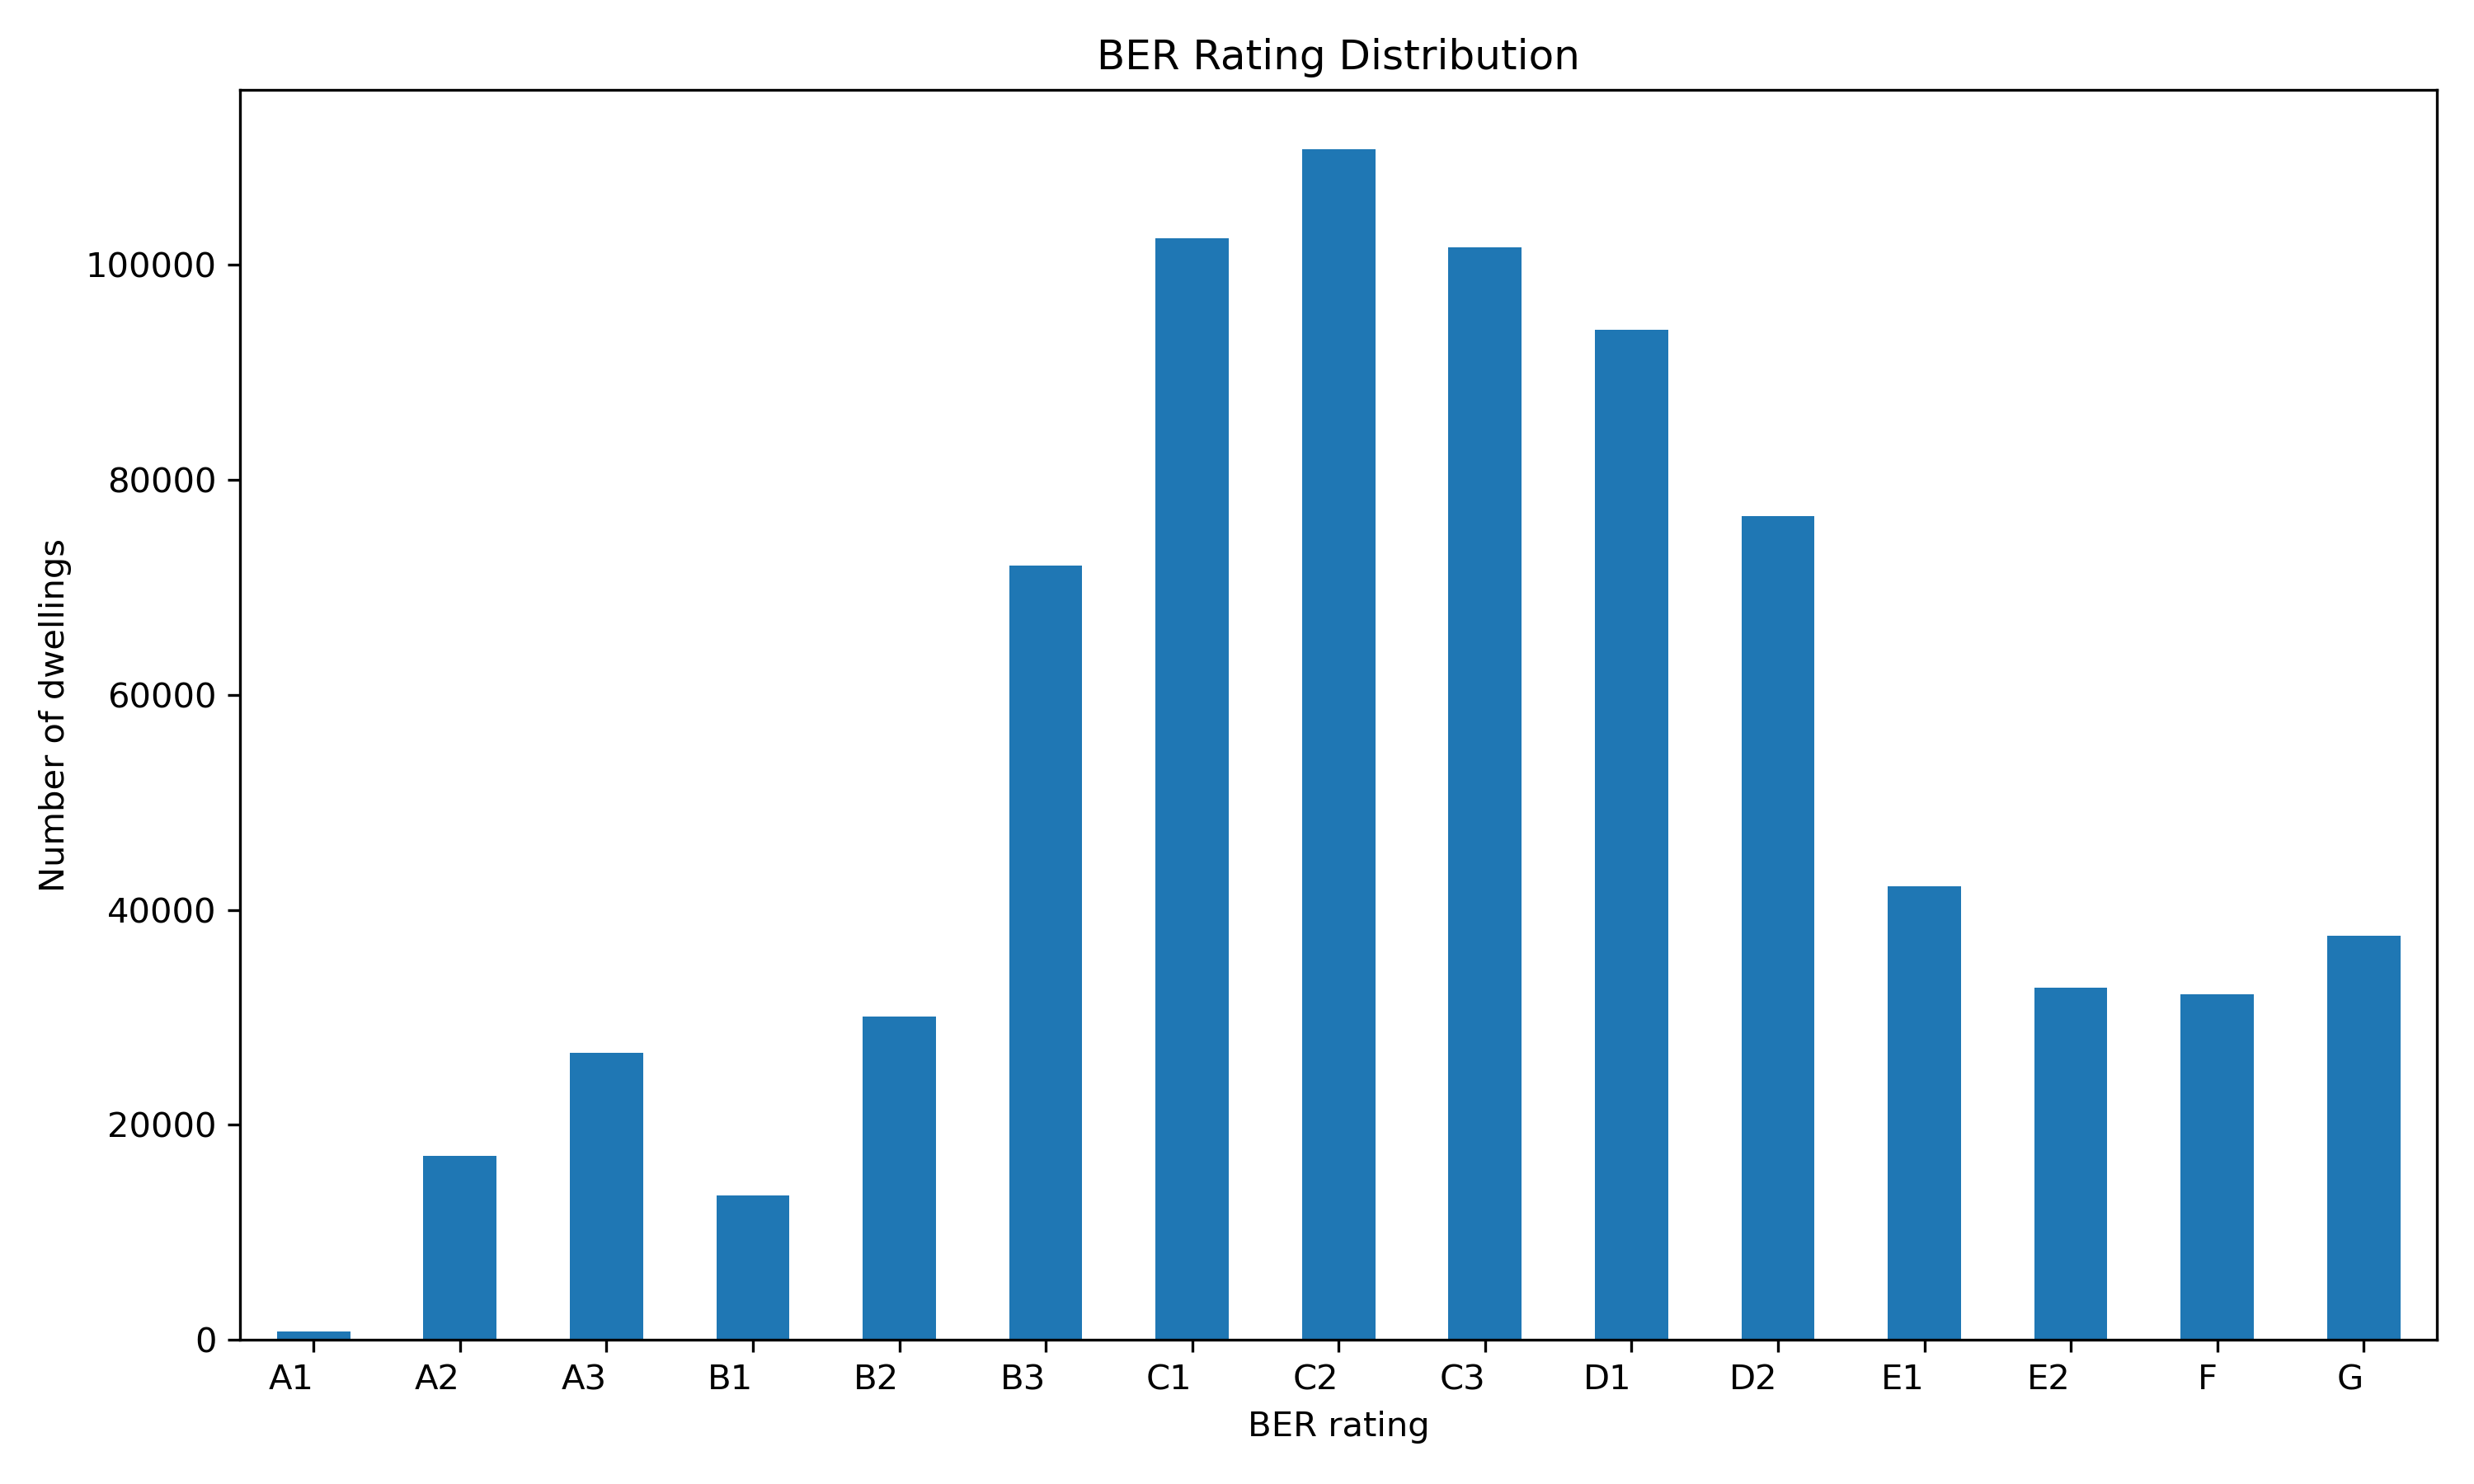
\includegraphics[width=0.9\linewidth]{figures/ber_rating_distribution.png}
\end{center}
\begin{itemize}
  \item Irish BER Database (cleaned), Ahern et al. (2024), Mendeley Data.
  \item \textbf{790{,}389} dwellings, 22 features after cleaning and a
  target-leakage audit (BER-derived output columns removed).
  \item Features: county, dwelling type, construction year, floor area,
  wall/roof/floor/window/door U-values and areas, heating fuels,
  glazing \%, volume.
\end{itemize}
}

\block{Target Definition -- Why B2?}{
\begin{center}
\begin{tabular}{@{}ll@{}}
\toprule
\textbf{Label} & \textbf{Condition} \\
\midrule
Not priority (0) & BER \textbf{B2} or better \\
Retrofit priority (1) & Worse than B2 \\
\bottomrule
\end{tabular}
\end{center}
\vspace{4mm}
\begin{itemize}
  \item Class balance: \textbf{88.8\% priority} vs 11.2\% not priority
  (imbalanced $\rightarrow$ balanced accuracy \& macro F1 used
  throughout, not raw accuracy).
  \item \textbf{B2 is not arbitrary}: it is SEAI's own recommended
  minimum retrofit standard, and the explicit target of the National
  Retrofit Plan -- \textbf{500{,}000 homes to B2 by 2030}.
  \item A model-flagged "priority" dwelling is, by definition, one that
  has not yet met the national retrofit benchmark.
\end{itemize}
}

\block{Methodology}{
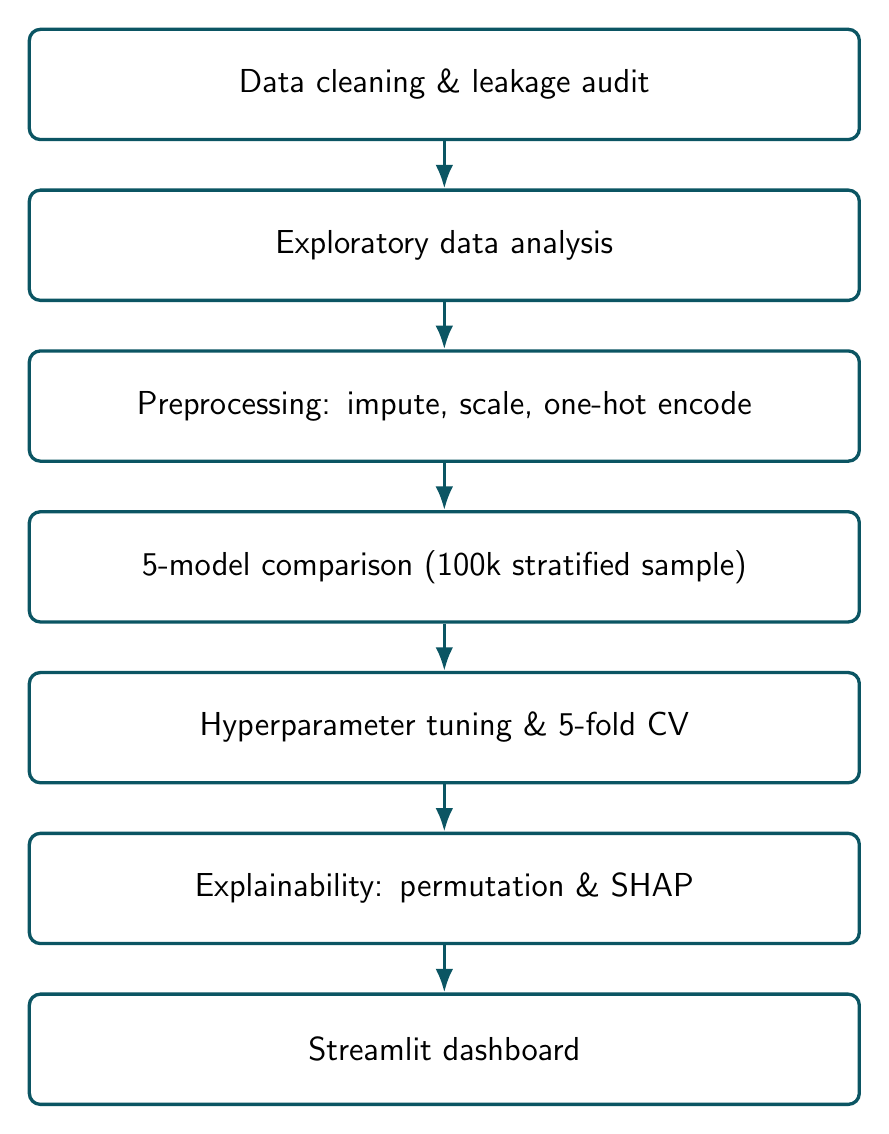
\begin{tikzpicture}[
  node distance=6mm,
  box/.style={rectangle, rounded corners, draw=posterTeal, very thick,
    fill=white, text width=0.85\linewidth, align=center,
    minimum height=14mm, font=\large},
  arr/.style={-{Latex[length=3mm]}, posterTeal, very thick}
]
\node[box] (n1) {Data cleaning \& leakage audit};
\node[box, below=of n1] (n2) {Exploratory data analysis};
\node[box, below=of n2] (n3) {Preprocessing: impute, scale, one-hot encode};
\node[box, below=of n3] (n4) {5-model comparison (100k stratified sample)};
\node[box, below=of n4] (n5) {Hyperparameter tuning \& 5-fold CV};
\node[box, below=of n5] (n6) {Explainability: permutation \& SHAP};
\node[box, below=of n6] (n7) {Streamlit dashboard};
\draw[arr] (n1) -- (n2);
\draw[arr] (n2) -- (n3);
\draw[arr] (n3) -- (n4);
\draw[arr] (n4) -- (n5);
\draw[arr] (n5) -- (n6);
\draw[arr] (n6) -- (n7);
\end{tikzpicture}
}

% ============================================================
% COLUMN 2
% ============================================================
\column{0.34}

\block{Model Comparison}{
Five models compared on a stratified 100k-row sample (80k train /
20k test): a majority-class dummy baseline, Logistic Regression,
Decision Tree, Random Forest, and Hist Gradient Boosting.

\begin{center}
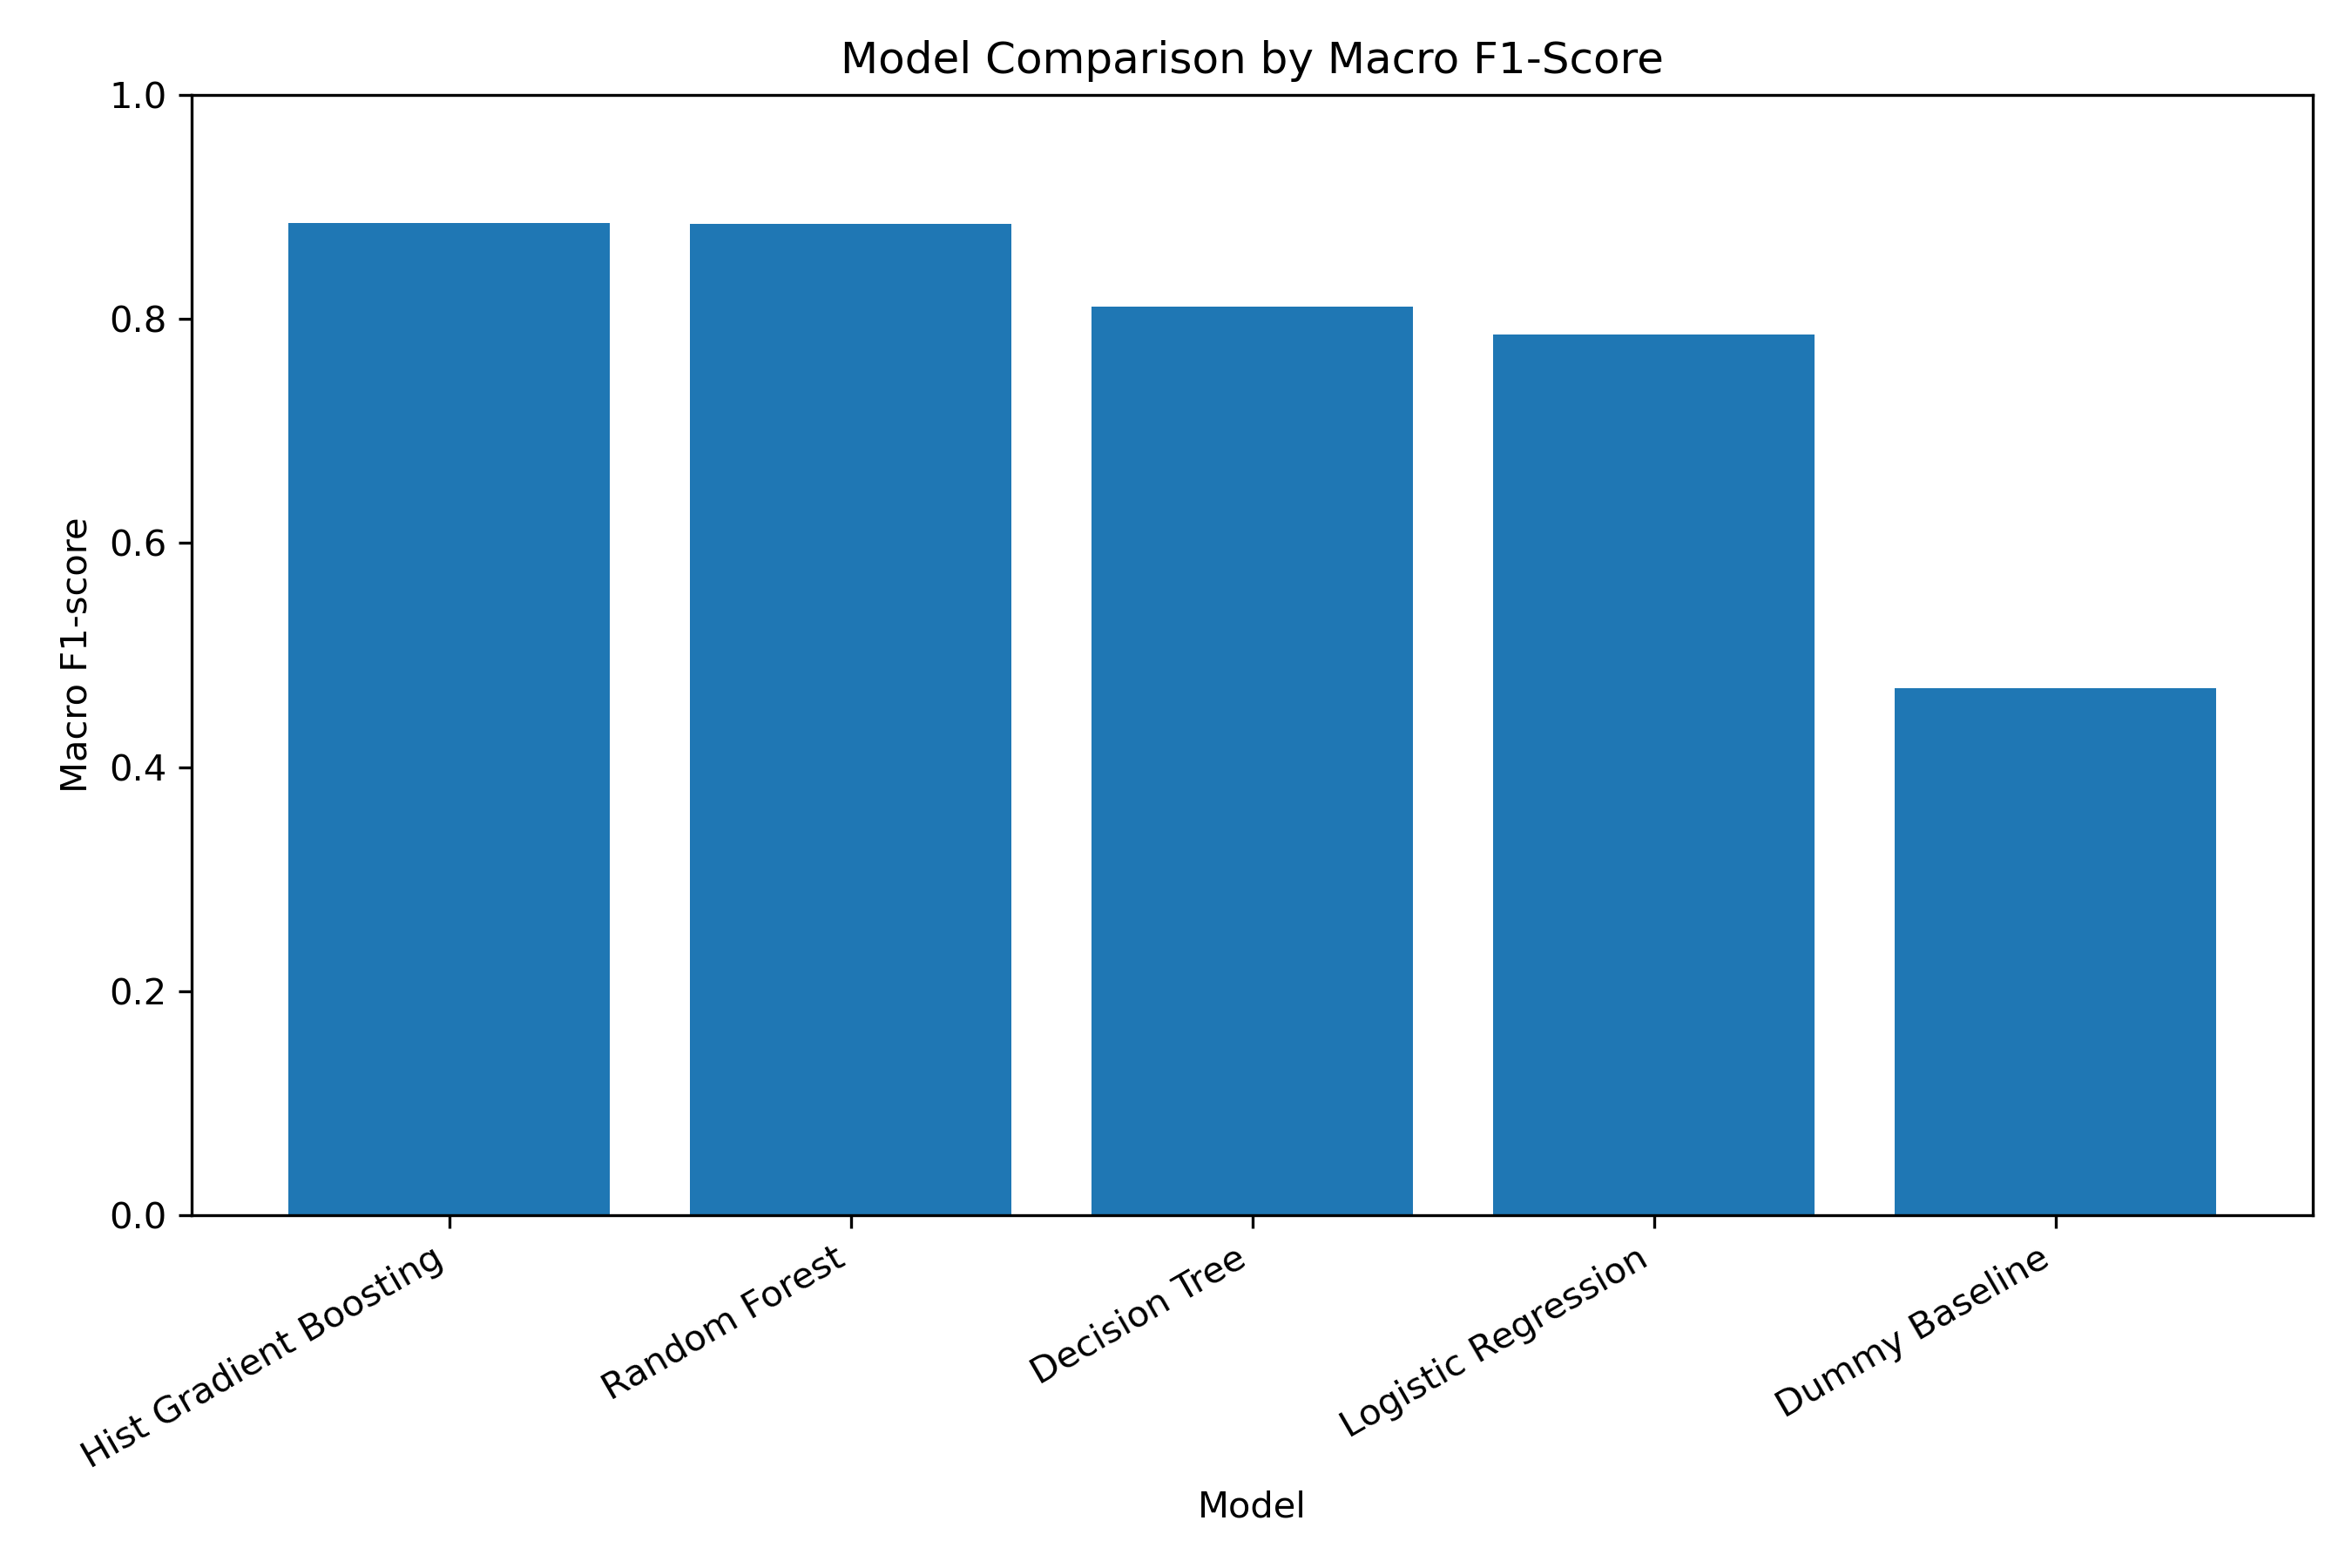
\includegraphics[width=0.95\linewidth]{figures/model_comparison_macro_f1.png}
\end{center}

\begin{itemize}
  \item The dummy baseline reaches 88.8\% \emph{accuracy} by always
  predicting the majority class -- but scores \textbf{0.50 balanced
  accuracy and 0.50 ROC-AUC}: no real discrimination ability.
  \item \textbf{Hist Gradient Boosting} gave the strongest overall
  trade-off (macro F1, ROC-AUC, high priority recall) and was selected
  as the final model.
\end{itemize}
}

\block{Tuning \& Validation}{
\begin{itemize}
  \item \textbf{RandomizedSearchCV}: 25 candidates $\times$ 5-fold CV,
  scored on macro F1, over learning rate, iterations, leaf count,
  min.\ samples/leaf, and L2 regularisation.
  \item Tuning improved every held-out metric except priority recall
  (a negligible $-$0.0004 change).
  \item \textbf{5-fold stratified CV} on the training split confirms
  the single test-split result is not a lucky draw: macro F1
  $= 0.886 \pm 0.005$, closely matching the 0.892 test-set score.
\end{itemize}

\vspace{3mm}
\begin{center}
\small
\begin{tabular}{@{}lrrrr@{}}
\toprule
& \textbf{Acc.} & \textbf{Bal Acc} & \textbf{F1} & \textbf{AUC} \\
\midrule
Default & 0.959 & 0.854 & 0.886 & 0.969 \\
\textbf{Tuned (final)} & \textbf{0.960} & \textbf{0.863} & \textbf{0.892} & \textbf{0.970} \\
\bottomrule
\end{tabular}
\end{center}
}

\block{Does Sample Size Matter?}{
\begin{itemize}
  \item Final model re-trained from scratch on 100k, 300k, and the
  \textbf{full 790{,}389-row} dataset (same tuned hyperparameters).
  \item Full-dataset training took under \textbf{40 seconds} --
  Hist Gradient Boosting scales well.
  \item Every metric improves modestly and monotonically with more
  data (macro F1: 0.892 $\rightarrow$ 0.904 at full scale) --
  confirming results are not an artefact of the smaller sample.
\end{itemize}
}

% ============================================================
% COLUMN 3
% ============================================================
\column{0.33}

\block{Explainability: SHAP \& Permutation Importance}{
\begin{center}
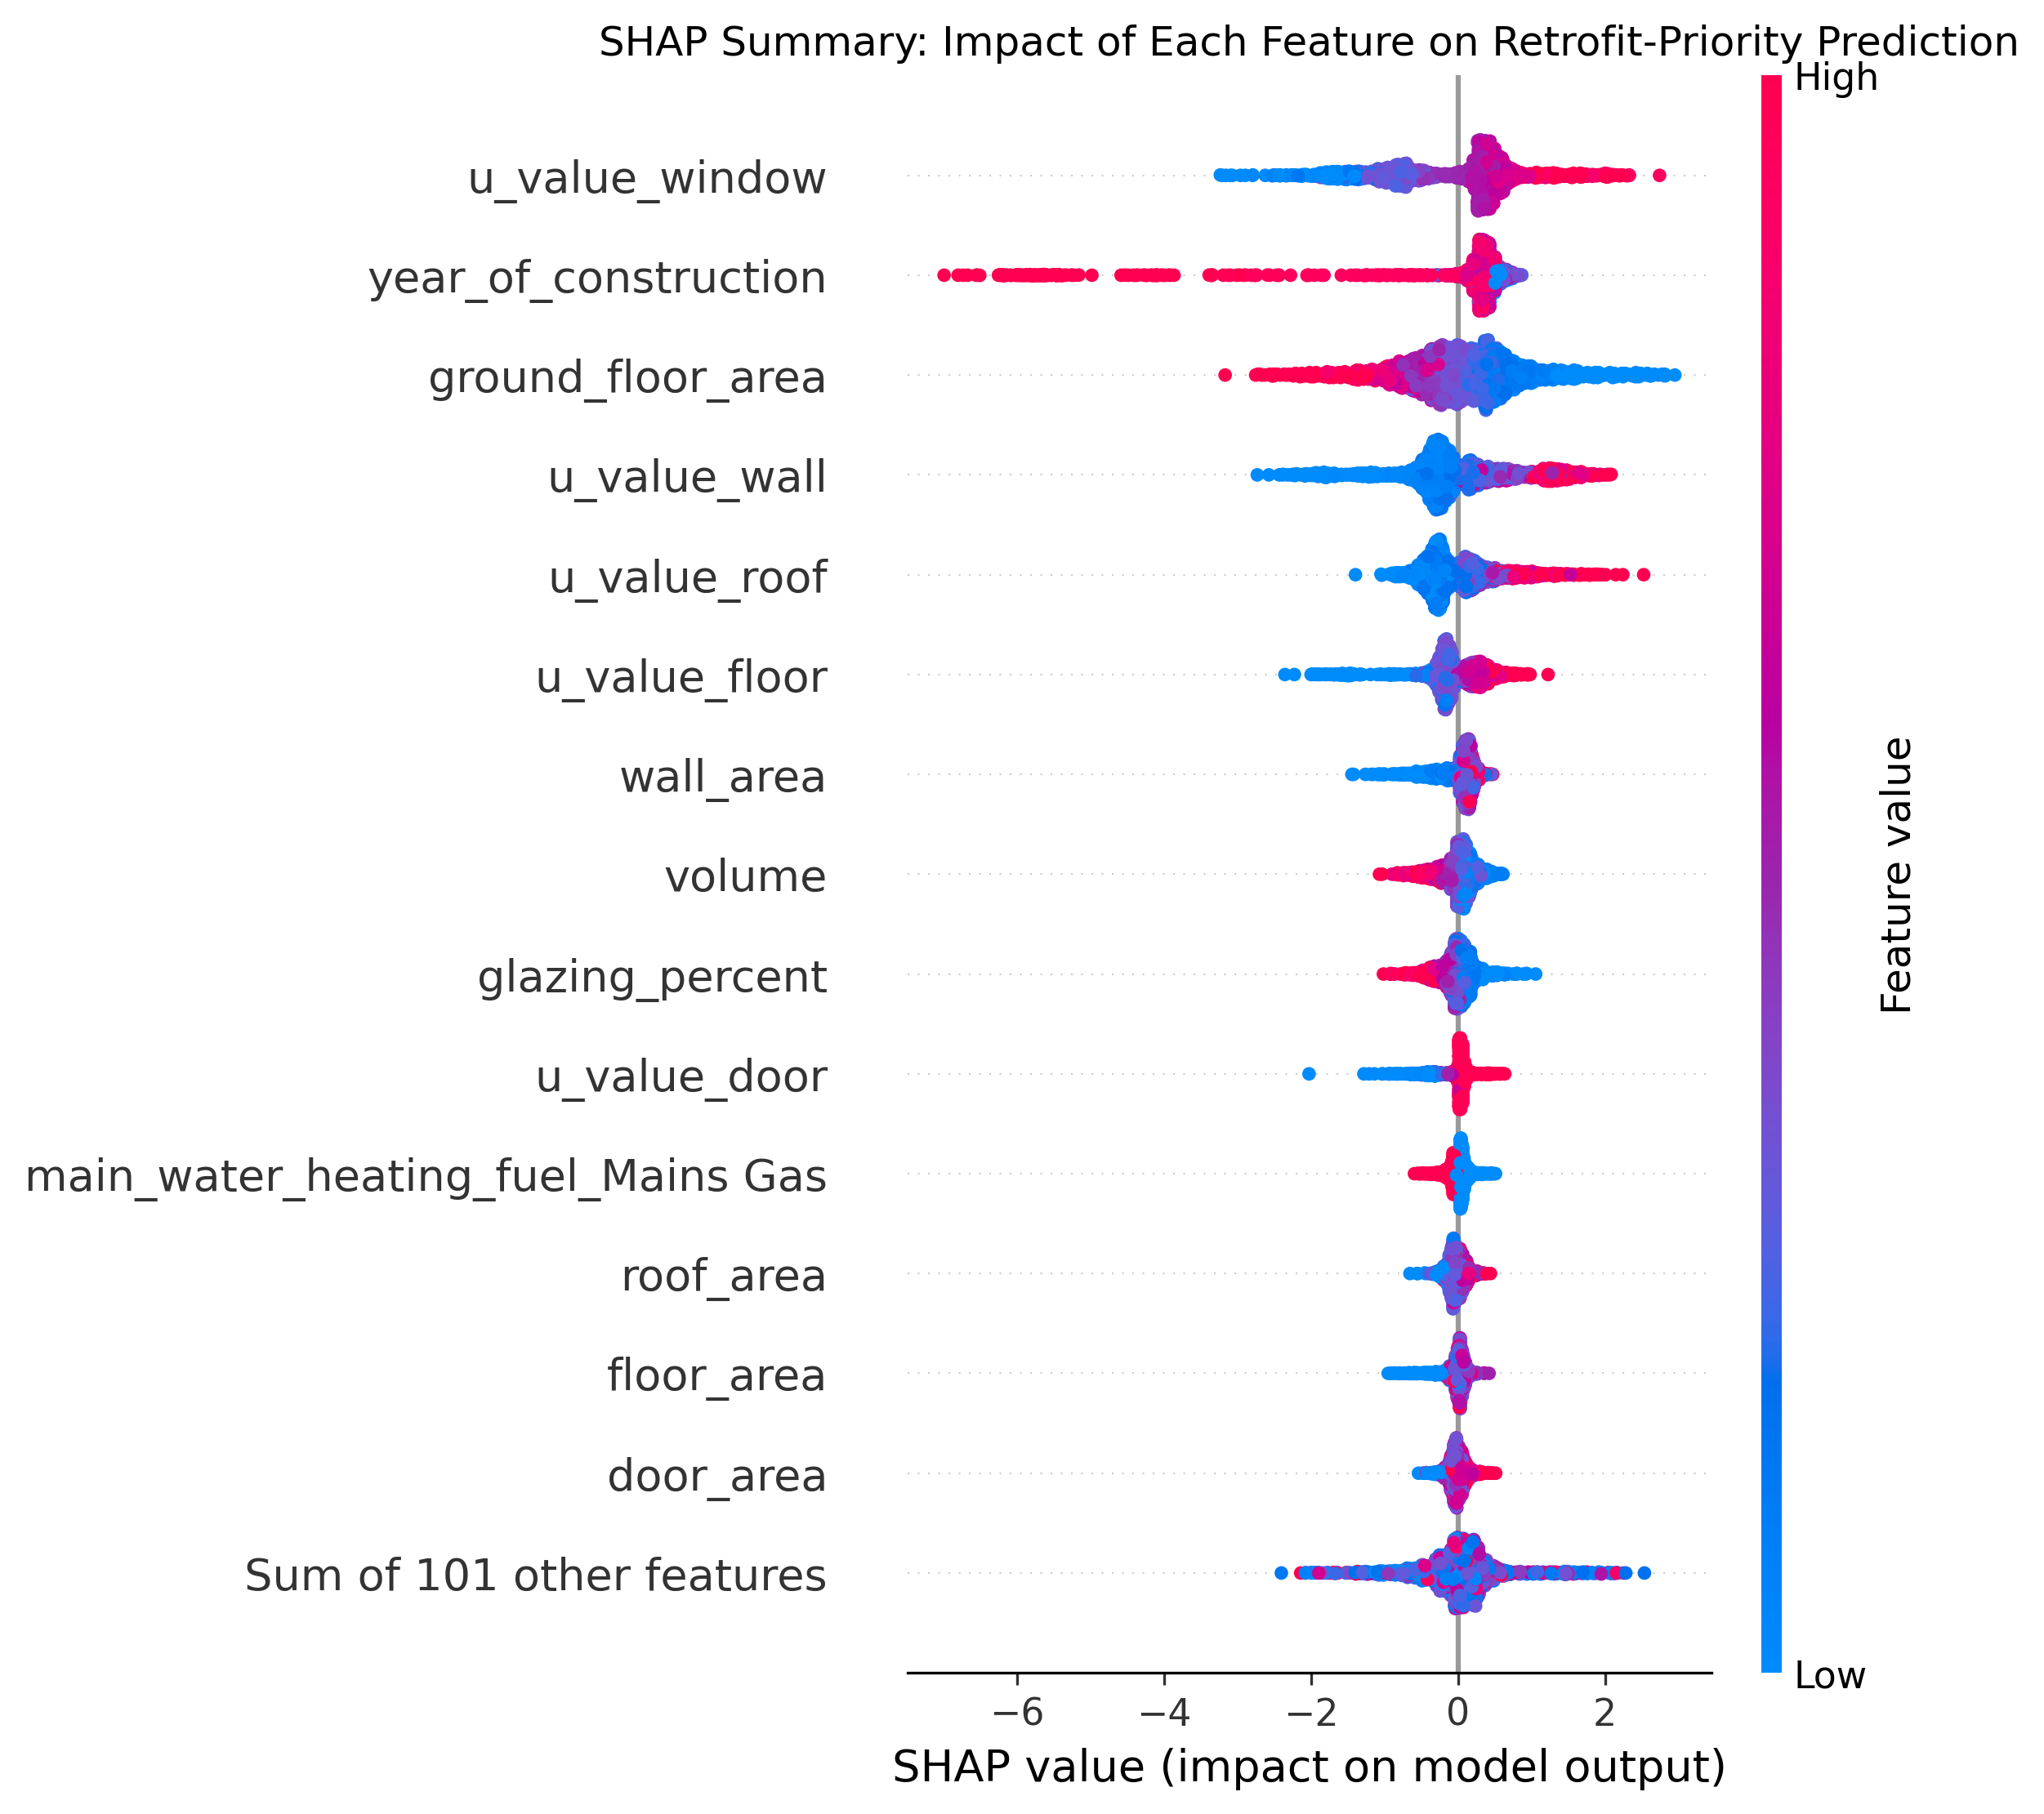
\includegraphics[width=0.95\linewidth]{figures/shap_summary_beeswarm.png}
\end{center}
\begin{itemize}
  \item Two independent methods agree closely: \textbf{8 of the top 10}
  features are shared between permutation importance and SHAP.
  \item Top drivers: \textbf{window, wall, and roof U-values},
  \textbf{ground floor area}, \textbf{year of construction}, and
  \textbf{water-heating fuel} -- all physically meaningful,
  consistent with building-energy principles.
  \item High (red) U-values push predictions toward retrofit priority;
  low (blue) U-values push toward not-priority -- exactly the expected
  physical direction.
  \item SHAP also explains \emph{individual} predictions in real units
  (e.g.\ actual U-values, m$^2$), not standardised model inputs --
  used live in the dashboard below.
\end{itemize}
}

\block{Key Interpretation}{
BER data predicts retrofit priority with strong performance
(\textbf{96\% accuracy, 0.97 ROC-AUC}), and the features driving those
predictions are exactly the ones building scientists would expect:
envelope heat loss, construction age, and heating systems -- not
arbitrary statistical artefacts.
}

\block{Interactive Dashboard}{
A Streamlit app puts the model in front of a user, not just a report:
\begin{itemize}
  \item \textbf{Predict} -- full input form for a dwelling's
  characteristics; returns the retrofit-priority prediction,
  probability, and a live SHAP waterfall explaining that specific
  prediction.
  \item \textbf{Model \& Data} -- comparison tables and key figures,
  doubling as a project showcase.
  \item \textbf{About} -- project summary, data source, and
  limitations for a general audience.
\end{itemize}
Scan the QR codes above the title to try the live app or browse the
full source code.
}

\block{Limitations \& Future Work}{
\begin{itemize}
  \item Binary label simplifies a continuous energy measure at one
  cutoff -- a D1 and a G-rated home are both "priority".
  \item BER reflects standardised assessment assumptions, not measured
  household energy use.
  \item Associations identified here are statistical, not causal.
  \item \textit{Future:} multi-level thresholds, county/dwelling-type
  specific models, full-dataset production pipeline.
\end{itemize}
}

\block{References}{
\footnotesize
Ahern, Raushan \& Essien-Thompson (2024). \textit{Irish BER Database
(Cleaned)}. Mendeley Data. DOI: 10.17632/yhgdzfpnym.1 \,\textbar\,
SEAI, B2 Home Energy Rating \,\textbar\, Government of Ireland,
National Retrofit Plan \,\textbar\, Lundberg \& Lee (2017), \textit{A
Unified Approach to Interpreting Model Predictions}, NeurIPS.
}

\end{columns}

\end{document}
